\providecommand{\main}{..}
\documentclass[\main/thesis.tex]{subfiles}

\onlyinsubfile{\zexternaldocument*{\main/tex/main chapter}}


\definecolor{codegreen}{rgb}{0,0.6,0}
\definecolor{codegray}{rgb}{0.5,0.5,0.5}
\definecolor{codepurple}{rgb}{0.58,0,0.82}
\definecolor{backcolour}{rgb}{0.95,0.95,0.92}

\lstdefinestyle{mystyle}{
    backgroundcolor=\color{backcolour},   
    commentstyle=\color{codegreen},
    keywordstyle=\color{magenta},
    numberstyle=\tiny\color{codegray},
    stringstyle=\color{codepurple},
    basicstyle=\ttfamily\footnotesize,
    breakatwhitespace=false,         
    breaklines=true,                 
    captionpos=b,                    
    keepspaces=true,                 
    numbers=left,                    
    numbersep=5pt,                  
    showspaces=false,                
    showstringspaces=false,
    showtabs=false,                  
    tabsize=2
}


\lstset{
    style=mystyle,
    columns=fullflexible,
    basicstyle=\ttfamily,
    frame=tlbr,
    framerule=0pt,
    xleftmargin=17pt,
    framexleftmargin=17pt,
    framexrightmargin=5pt,
    framexbottommargin=4pt,
    aboveskip=20pt,
    belowskip=20pt
}
    

\begin{document}

\chapter{Main Chapter}

SIMD intructions allow modern processor to apply the same Intruction on multiple data at the ame time. The performance improvement gained from these intructions is 
so considerable(?) that made compiler specialists to explore different ways to exploite SIMD intructions. Auto-vectorization [cite] is a compiler tranformation that is proposed
for this purpose. Implemented by almost all current compilers, auto-vectorization looks for possibility of using SIMD instructions (also called vector instructions) in the program and replaces
scalar code (code that is made of simple instructions) with vector instructions wherever possible.

Since most of the execution time of a program is spent on loops, vectorization is typically applied on loops. Famous Compilers have optimization passes (such as slp-vectorizer in clang ... [cite, more examples])
that vectorize loops body. In spite of loop-vectorization there has been efforts to vectorize other structres such as functions [cite] as well however, the focus of research in this area is on loops.

A huge amount of work has been done to improve codes using vectorization [cite] however, the transformation needs the code to meet certain requirements which if not met, would result in invalid code
produced by the compilers. Furthuremore, replacing scalar code with vector is not always benefitial. In some situations(?) scalar code can provide better performance in comparison to vector code.
In response to these two problems with vectorization, compilers come with an analysis pass to check both legality of the tranformation and it's profitability.

One of the larget obstacles for vectorization has always been control flow divergence. Existence of branches (such as if-then-else statements or swithch case statements) causes the program to take different paths during execution time 
based on some conditions inside the code that could change dynamically. This is called divergence in the control flow of the program. Having divergence in the code, vectorization can not be simply applied,
as different iterations of the loop might take different paths and as a result disabling the compiler to replace instructions with SIMD ones. 

To deal with divergence in the code, a tranformation called If-Conversion (also called Control Flow Linearization)  has been proposed. Modern Processors support "predicated instructions". in predicated instructions, every single instruction is 
gaurded by a one bit predicate which could be either 1 or 0. The result of execution of the instruction will be committed only if that predicate bit is set to 1. Otherwise, the result will be discarded leaving no architectural(?) effect e.g: memory writes (?),... .
Having "Predicated Vector instructions" in the processor, compilers will be able to vectorize codes with divergence by first Linearizing control flow and then replacing scalar instructions with vectorized ones.
This is the most widely taken approach to vector such codes with divergence, But there are probelms with this approach.

To demonstrate possible shortcomings with this approach, let's follow a simple example: 

% \begin{algorithm}
%     \caption{Motivating Example}\label{euclid}
%     \begin{algorithmic}[1]
%     \For{$i \gets 0$ to $N$ by 1}
%         \If{($i \bmod $2) == 1} 
%             \State $C_{i} \gets $($A_{i} + B_{i}$) 
%         \Else
%             \State $B_{i} \gets $($A_{i} - C_{i}$) 
%         \EndIf 
%     \EndFor

%     \end{algorithmic}

% \end{algorithm}


\begin{lstlisting}[language=C, caption={Motivating Example}]
    for(i = 0; i < n; i++){
        if(cond[i]){
            a[i] = b[i] * c[i];
        }else{
            b[i] = a[i] + c[i];
        }
    }
\end{lstlisting}

There are two different paths inside the loop body which disable us to simply vectorize the code. As explaned before, we need to first linearize the control flow through if-conversion and then vectorized code. After doing so, resulting code 
would look like this:(In this section we assume that vector length is 4.)

\begin{lstlisting}[language=C]
    VLength= 4;
    for(i = 0; i < n; i+=VLength ){
        a_v = load_v(&a[i], VLength);
        b_v = load_v(&b[i], VLength);
        c_v = load_v(&c[i], VLength);
        mask_v = load_v(&cond[i], VLength);
        mult_v = masked_mul(b_v, c_v, mask_v);
        masked_store_v(&a[i], mult_v, VLength, mask_v);
        mask_not_v = not_v(mask_v);
        add_v = maked_add(a_v, b_v, mask_v)
        masked_store_v(&b[i],add_v, VLength, mask_not_v);
    }
\end{lstlisting}

When we apply if conversion, all branches are eliminated and instead, all instruction are gaurded with predicates. In line 6 we have computed the mask for instructions that belong to if block. Then instructions in lines 7 and 8 use this mask vectore. Since here we have a simple if then else statement,
the predicate for else block instructions will simply be negated(?) predicates we had for if block. So in line 9 we used not instruction to form mask vector for then block and used it for instructions in lines 10 and 11.

As you can see, by applying if conversion, we are always executing codes in both if and else blocks and because the conditions for these two blocks are mutually exclusive, no matter how many true and false elements exist in 
the mask vector, we always end up wastng half of vector lanes due to predication.

This problem has been studied for a while and recent works [cite] has proposed solutions for that. The main idea behind most of these solutions is to detect \textbf{Uniform True} and \textbf{Uniform False} paths.

A uniform path refers to the case where for one vector iterations, all predicates are either true or false which means all iterations are going to execute one path (in our motivating example either then block or else block). If such a uniform is detected, All we need to 
do is to introduce a path (coressponding to the block it's going to execute) that all instructions are vectorized but not predicated. Doing so we will: 1- utilize full vector capacity to execute code and 2- avoid excessive overhead introduced by predicated 
instructions.

Having the idea of uniform paths, the main challenge is how to detect uniform vectors. As discussed above and we saw in the example[figure number], predicated vectors are formed from branch (in the example the if statement) conditions. The value for these conditions could be 
either static or dynamic. In case of static, compiler could find its value at compile time and apply appropriate optimizations to produce the most performant(?) code however, in most cases the condition can only be determined at runtime and could change on each iteration and 
a result static approaches are unable to detec uniformity. 

Runtime checks are typical solutions to this problem. Compiler inserts some runtime checks to find if a vector is uniform in that execution time or not. Compiler also introduced some paths so that when a uniform vector is detected dynamically, the coressponding path will be executed.

To demonstrate how this approach works, let's apply it on the code in figure [FIG number]:

\begin{lstlisting}[language=C]
    VLength= 4;
    for(i = 0; i < n; i+=VLength ){
        a_v = load_v(&a[i], VLength);
        b_v = load_v(&b[i], VLength);
        c_v = load_v(&c[i], VLength);
        mask_v = load_v(&cond[i], VLength);
        if(all_true(mask_v)){
            /* uniform true path */
            mult_v = b_v * c_v;
            store(&a[i], mult_v, VLength);
        } else if (all_false(mask_v)){
            /* uniform false path */
            add_v = a_v + c_v;
            store(&b[i],add_v, VLength);
        }else{
            /* Linearized Path */
            mult_v = masked_mul(b_v, c_v, mask_v);
            masked_store_v(&a[i], mult_v, VLength, mask_v);
            mask_not_v = not_v(mask_v);
            add_v = maked_add(a_v, b_v, mask_v)
            masked_store_v(&b[i],add_v, VLength, mask_not_v);
        }
    }
\end{lstlisting}

Like before, we formed mask vector in line 6. Then we check to see if all elements in mask vector is true. If so, it means that we have detected a uniform vector coressponding to if blcok and we can execute if code without predication. But if the all elements of the mask are false, then we have detected 
uniform vector coressponding to else block. So we can execute else code with no predicatation. Otherwise, it means that the vector is a combination of true and false elements which execute different paths in the code (some if block and some else). In this case we use predicated code in our linearized path as before.

Although uniform paths could possibily lead to performance improvement, there are two things to consider about them: First, they introduce overheads due to runtime checks they add to the code and second, if the input is in a way that uniform vectors are unlikely to occur, then unifrom paths
won't be executed often, thus no improvement will be gained.

Wytte[cite] suggested the idea of \emph{forming} uniform vectors reather than \emph{waiting} for one to occur. He proposed his transformation called Active-Lane-Consolidation (ALC) to dynamically form such uniform vectors. The main idea behind this transformation is to \emph{permute} loop indices
so that eventually we have a uniform vector of indices which then executes the coressponding block without preication. 

To see how it works let's apply it to our motivating example in figure[?]:
\begin{lstlisting}[language=C]
    VLength= 4;
    /*Initialization*/
    uniform_vec = index(0,VLength);
    uniform_mask = load_v(&cond[0], VLength);
    for(i = 0; i < n; i+=VLength ){
        index_vec = index(i, VLength);
        mask_vec = load_v(&cond[i], VLength);
        uniform_vec, remaining_vec, uniform_mask, remaining_mask = Permute(uniform_vec, index_vec, uniform_mask, mask_vec);        
        if(all_true(uniform_mask)){
            /* execute if block without predication */
            b_v = gather_load_v(&b, uniform_vec);
            c_v = gather_load_v(&c, uniform_vec);
            mul_v = b_v * c_v;
            scatter_store(&a, uniform_vec, mul_v);

            uniform_vec = remaining_vec;
            uniform_mask = remaining_mask;
        }else {     
            /* execute else block without predication */
            a_v = gather_load_v(&a, remaining_vec);
            c_v = gather_load_v(&c, remaining_vec);
            add_v = a_v + c_v;
            scatter_store(&b, remaining_vec, add_v);
        } 
    }
\end{lstlisting}

In lines 3 and 4, the uniform vector (uniform\_vec) and its mask vector (unifrom\_mask) have been Initialized with indices 0 to VLength and the coressponding masks respectively.
Then in each iteration of the loop, next vector of indices and its masked vector have been formed. The magic happens in line 11 where we call the permute function. It will put all active elements in uniform\_vec, the other elements in remaining\_vec and coressponding mask bits to uniform\_mask and remaining\_mask.
After doing so we check if all mask bits in uniform\_mask is true. If this happens, it means that we have formed a uniform vector coressponding to then block and we can execute it with no predication. Otherwise, we are sure that all mask bits in remaining\_vec is false thus, without checking this condition we can 
execute else block with indices stored in remaining\_vec vector, again with no predication.

As we can see, using ALC, we always have a uniform (either uniform true for uniform false) vector in each iteration and there is no need to use predicated instructions anymore. 

The only part of code that can affect the performance negatively is Permute function. If Implemented naively, it could result in even worse performance that predicated code. This is why Wytte propsed his transformation only for ARM architecture with SVE support. SVE (Scalable Vector Extention)[cite] is a vector extention
proposed by ARM that provides special vector instructions that makes it possible to Implement different vector algorithms efficeintly (elaborate more on sve). Using these instructions, Wytte proposed a fast algorithm for permutation [cite].

In this work we continue his work on ALC. He proposed the idea of ALC and showed that it could be benefitial by manualy applying it on some selected benchmarks however, he just ran his experiments on a simulator that could only count dynamically executed instructions. This is because at the time there very few machines 
that supported SVE instructions. His results showed that applying ALC on the cases where he thought would be benefitial, could result in significant reduction in dynamically executed instructions compared to scalar code and also considerable reduction compared to vectorized code.

We argue that although such a result is promising, it's not enough to demonstrate that the optimization is actullay benefitial. Vector instructions by nature reduce the number of instructions executed as they operate on multiple data at the same time but they also introduce more overheads in terms of latency. 

The other important aspect that could be severely imapcted by ALC transformation is cache misses. When a load/store happens to a memory address, proccessor also loads data from adjacent memory addresses to the cache since it's likely that it will be used by next operations, which is called locality. Having a memory access patteren in the code that 
utilizes the memory locality is essential to provide performance however, ALC is so likely to change this access pattern by accessing different memory addresses through \emph{gather load} and \emph{scatter store} instructions. It is apparent that such behaviours their imapct on performance can not be easily detected through metrics such as executed instructions.

In this work we propose a compiler pass that automatically applies ALC tranformation on a given code. Such an automatation requires a deep analysis of first legality of the tranformation and second costs and expected benefits of it. To answer this requirement, our pass comes with an intesive (?) analysis phase that is executed before any tranformation is done. Next, 
we improve ALC algorithm by proposing different versions of it. Analyzing Wytte's results we found that the same approach for ALC is not able to provide benefits for every case however, small modifications to the algorithm and new versions of it could provide good performance improvements. So we tried to first deivide input codes structures to different categories and
propose different versions of ALC each specialized for that category.

Having the analysis phase and different versions of ALC, we combine them together to offer a solid recipe for ALC tranformation that can now automatically be applied on every input code and expect improvements.


\section{ALC Strategies}

In this section we explain how we do the transformation for each case. We start by Wytte algorithm, show the potential cases where it would not result in good performance. Then we analyze what is happening in detail to fine the solution and propose our modified version which works well.

\subsection{If-Then-Else Case}
It's worth first talking about the hypothesis behind ALC performance improvement. When we linearize and then vectorize the code with control flow divergence, what happens is that in each iteration of the loop we are adding two sources of overhead:
\begin{enumerate}
    \item The overhead of predicated instructions
    \item redundant computations which their results will be discarded later 
\end{enumerate}

The first one is quite clear. Proccessor can execute normal instructions faster than predicated ones since it need to keep track of the predicates to decide whether it should commit the changes or not.

To better understand the second problem let's consider our motivating example on figure ?? and assume the if condistion is going to be true on every other iteration. So in total, half iteration will execute then block and the other half will execute else block.
now lets move to the figure ?? where lineariation and vectorization have been applied to the code. Let's focus on the first iteration of the vectorized loop.


\begin{figure}[t!]
    \centering
    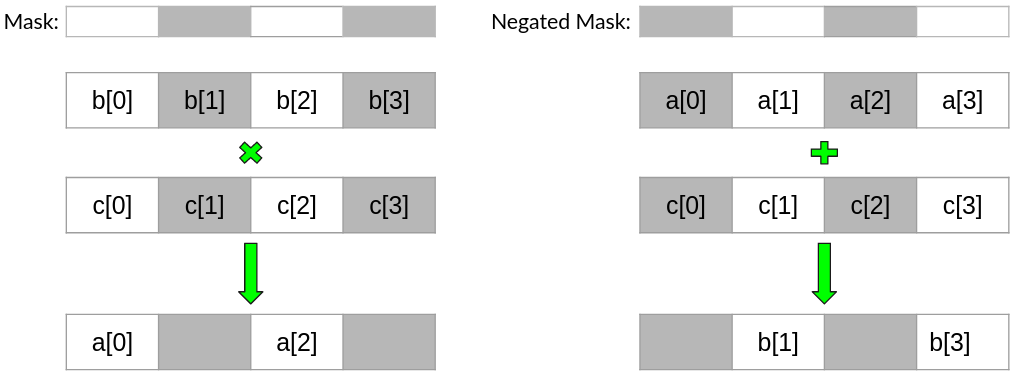
\includegraphics[width=0.95\textwidth]{img/masked_operations.png}
    \caption{Masked Opertions}
    \label{fig:masked_multiplication}
\end{figure}

After vectors \emph{a\_v, b\_v, c\_v} are loaded in lines 3-5, the mask vector is formed which we know in this example, will be true for \emph{first} and \emph{third} elements and will be false for \emph{second} and \emph{forth} elements. figure ?? illustrates what will happen at lines 7 to 11 of the code. White elemets are the ones coressponding to true mask and gray ones coresspond to false mask.
For each Opertion, the vector unit of the processor will do the operation for all lanes \emph{regardless} of mask values. After doing so, it will discard result for false elements and only keep the true ones and then store them to the memory. Vector instruction could have significant more latency [cite?] compared to scalar instructions and as you can see, we are wasting half our computation power while paying the overhead of vector instructions in each iteration.

In the this example we supposed that the confdtion is true every other iteration but when we have if and else blocks, any sort of distribution of the true and false conditions would have the same impact. Figure ?? shows different possible scenarios which might happen in each iteration of the if-converted code at runtime. It assumes that numbers of instructions in both if and else blocks are the same. The green elements correspond to active elements of the vector exectuing then block 
instructions and blue ones are those corresponding to active elements of the vector exectuing else block. The gray ones show inactive lanes. As you can see, regardless of how predicates look like, we always endup wasting half vector elements in total as long as then and else block are approximately of the same size. 

\begin{figure}[t!]
    \centering
    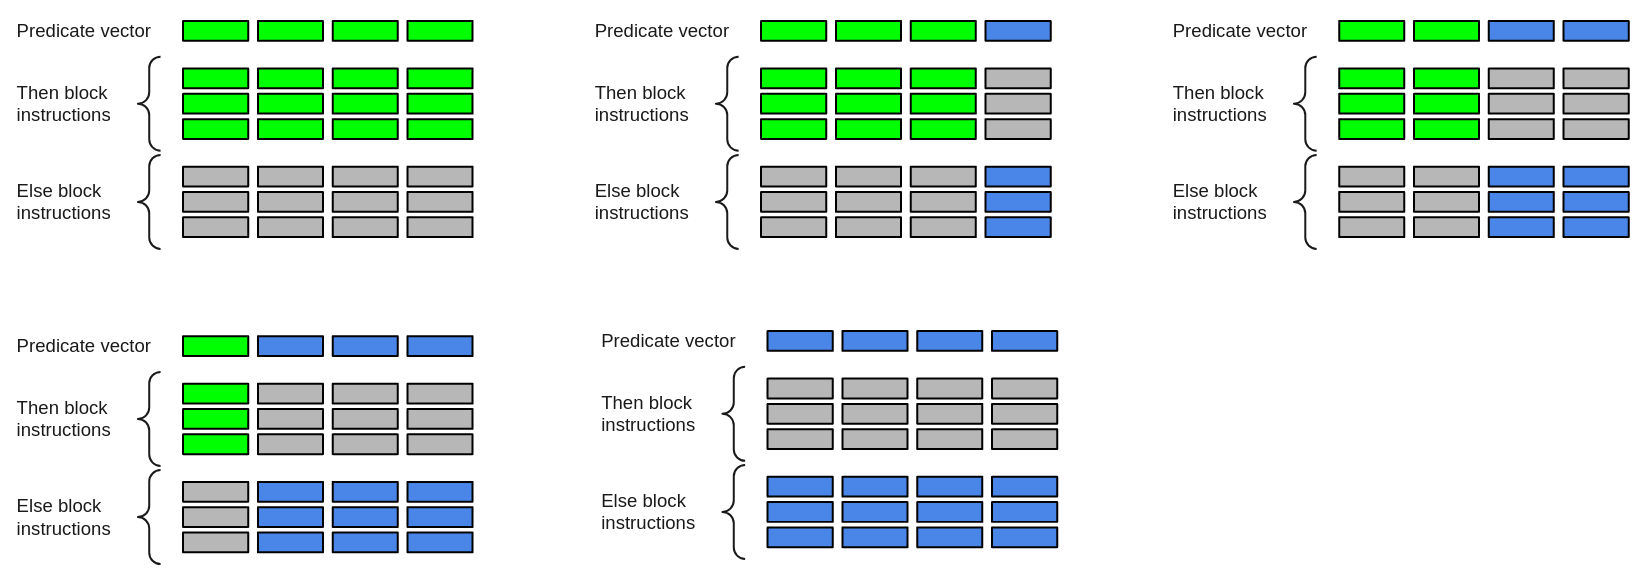
\includegraphics[width=0.95\textwidth]{img/condition_distribution.png}
    \caption{different scenarios for predicate distribution}
    \label{fig:predicate_distribution}
\end{figure}

The idea behind ALC is to utilize vector instructions by postponing any masked operation to the point where, we have a uniform vector filled with all active lanes. This way not only we don't waste any computation power but we also eliminate maksed operation which are more expensive that regular ones as discussed before.

To accomplish this, we use vector permutation algorithm proposed by Wytte[cite]. The high level view of this operation is illustrated in fig(?). White color represents vector elements for which the coressponding predicate is true (we call them active lanes of the vector) and the gray ones show elements coressponding to false predicates (we call them inactive lanes).
Given two predicated vector, the permutation logic fills the first vector with active lanes, and puts the other ones in the second vector. If there are enough active lanes in both vectors to fill the first vector, permutation will produce a uniform true vector and if not, then the total number of inactive lanes is more than the size of a vector and permutation will produce
a uniform false vector. As a result, no matter how the input vector look like, after doing the permutation, we will have \emph{at least} one uniform vector.

\begin{figure}[t!]
    \centering
    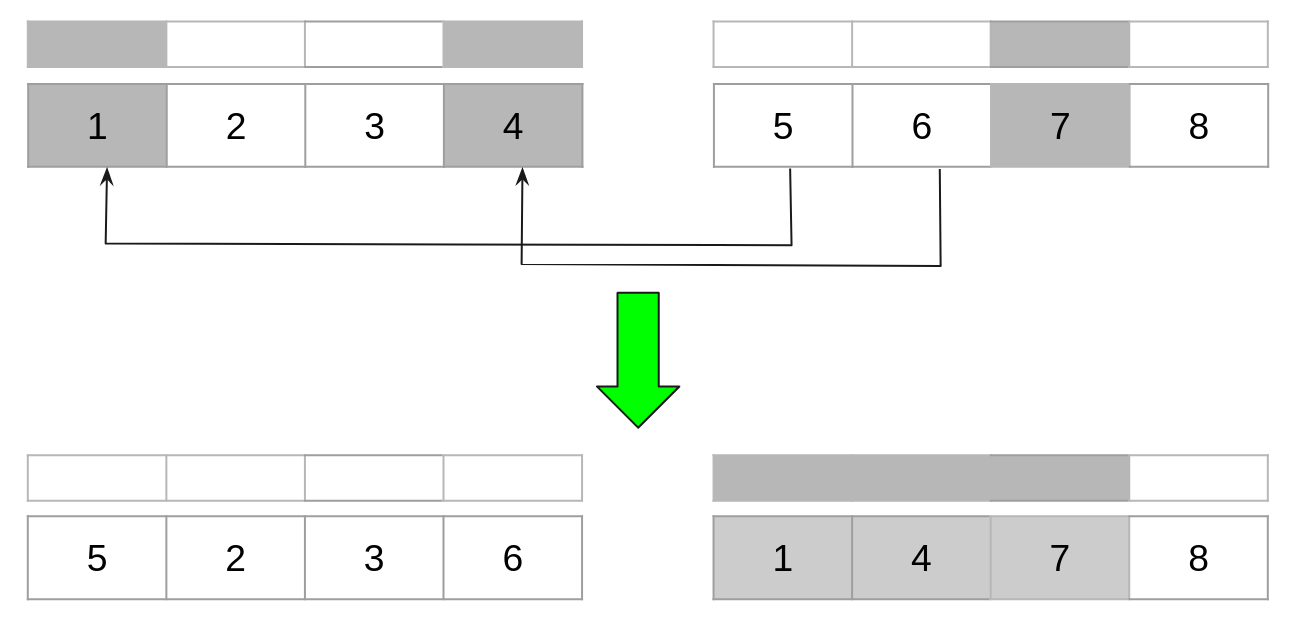
\includegraphics[width=0.90\textwidth]{img/permutation.png}
    \caption{Permutation Logic}
    \label{fig:permutation}
\end{figure}

Having the permutation algorithm, we implemented what wytte calls \emph{Iterative ALC} as a compiler pass. High level approach is illustrated in figure(?).

In this version of ALC, vectors contain indices of the loop, so we also call it \emph{index permutation}. In each iteration, we have two vector of indices, one the indices of current loop iteration and the other one, indices of previous iterations that have not been executed yet. ALC starts by permuting these two vectors, forming a uniform vector. If it produces a uniform true vector, then it will execute 
Then block for those elements. Otherwise, as discussed before, we have a uniform false vector and we execute the else block for those indices. No matter which block executed, the other vector (which could have any combination of true and false elements) is passed to the next iteration for permutation.


\begin{figure}[t!]
    \centering
    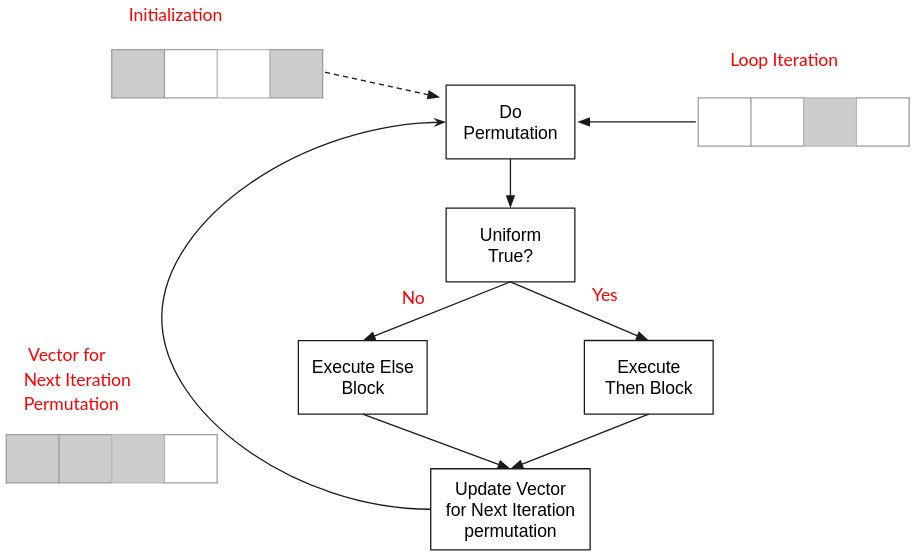
\includegraphics[width=0.95\textwidth]{img/iterative_alc.png}
    \caption{High Level approach for Iterative ALC}
    \label{fig:iterative_alc}
\end{figure}

You have probably noticed the trade-off in ALC. We add the overhead of index permutation but in return, we avoid predicate instructions and fully utilize proccessor computation power. The cost of permutation is independant from the size of the loop and instructions it has. The only factors that affects it is loop trip count (number of times loop is going to be executed) as it determines how many times the permutation should happen.
So you can see that as number of instructions inside the loop increase, the overhead of permutation becomes smaller compared to the overhead of loop instructions and ALC makes more sense. As a result, there should be a threshold of(?) minimum number of instrcution in the loop to apply ALC. We will exaplain this in details in Analysis section.

In order to compare the performance of ALC and vectorization applied by state-of-the-art compilers, we provided a simple test shown in fig(?). It consists of a single loop which contains an if-then-else statements. there are a large number of load/store and arithmetical instructions inside the e\emph{then} and \emph{else} blocks so that it overcomes the overhead of permutation. Figure (?) shows The speed up of each version over scalar code.
For the scalar code, we compiled code with \emph{Clang} compiler disabling \emph{vectorization} and \emph{loop-unrolling}. As you can see, although ALC brings a speedup of around 2.9X, it is still slower than Armclang by almost 5/%.



\begin{figure}[t!]
    \centering
    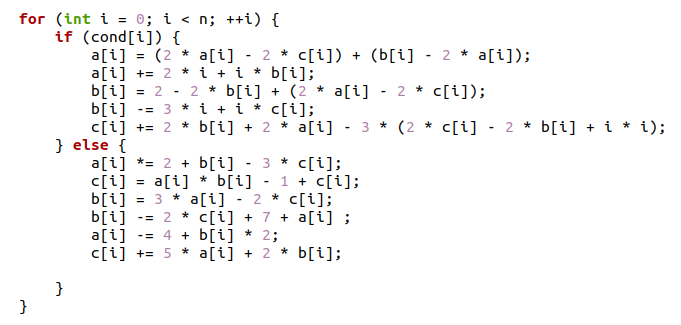
\includegraphics[width=0.95\textwidth]{img/test.png}
    \caption{test code to comapre ALC and Armclang}
    \label{fig:iterative_alc}
\end{figure}



\begin{figure}%
    \centering
    \subfloat[\centering Speedup over scalar code]{{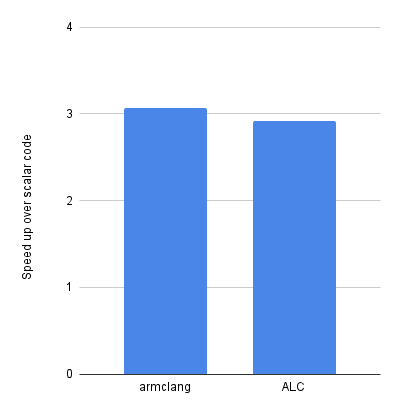
\includegraphics[width=5cm]{img/alc_vs_armclang_test_cycle.png} }}%
    \qquad
    \subfloat[\centering Number of cycles stalled for memory operations]{{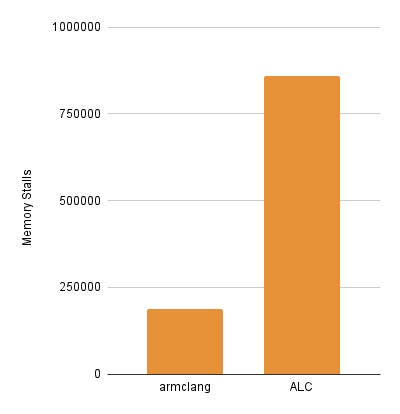
\includegraphics[width=5cm]{img/memory_stalls.png} }}%
    \caption{Comparison between Armclang vectorization and ALC}%
    \label{fig:example}%
\end{figure}




\section{Analysis Phase}

The analysis has three major roles:
\begin{enumerate}
    \item To make sure that for the given loop we are allowed to apply ALC.
    \item How does the structure of CFG look like and chooses the right approach for Apply ALC.
    \item Based on the information it gathers, is it benefitial to do the tranformation or not.
\end{enumerate}

As Wytte explained in his work, in order to be alowed to apply ALC which means that we need to make sure that the generated code will be correct and the result of the execution will be exactly the same as the result for exectuing scalar code, we must make sure that the loop has no function calls, no loop carried dependecy and there exists at least two paths inside the loop. The first responsiblity of the analysis is to check these restrictions.

Providing a general recipe to do the tranformations for any input code requires gathering infromation about exact structure of control flow, so that we can classify any sort of divergence in a pre-defined category. To attain this goal we first define three categories of divergence
which will cover all possible shapes of control flow. Having them classifed, we can then propose techniques and algorithms for applying ALC in each case. The three categories are followings:

\begin{enumerate}
    \item Single if statement.
    \item Single if-then-else statement.
    \item Any divergene with more that 2 control flow paths.
\end{enumerate}

There are different experimental factor that lead us to these three categories which include the level of difficulty to apply the pass and expected improvement for each case. The recipe to apply the transfromation on each case is explaned in next chapters.

Finally, After making sure that we are allowed to apply ALC and finding the right categoriy for the loop, we need to make the dicision of whether it's benefitial to do the tranformation or not. This is one the most challenging parts since the improvement that comes from the ALC depends on several different factors which some of them could be detected only at run time. In Section ?? we will explain these factors and requirements and how our cost model answers them in detail.   


\end{document}